Le combat était la partie du moteur de jeu la plus compliquée à implémenter.
Il fallait combiner plusieurs tableaux complexes avec des relations très spéciales entre eux.
Ceci bien sûr pour ordonner à des unités dans un hexagone d'attaquer des unités ennemies dans un hexagone adjacent.
Nous pouvons voir ci-dessous le tableau fourni dans les règles du jeu:

\begin{figure}[H]
\centering
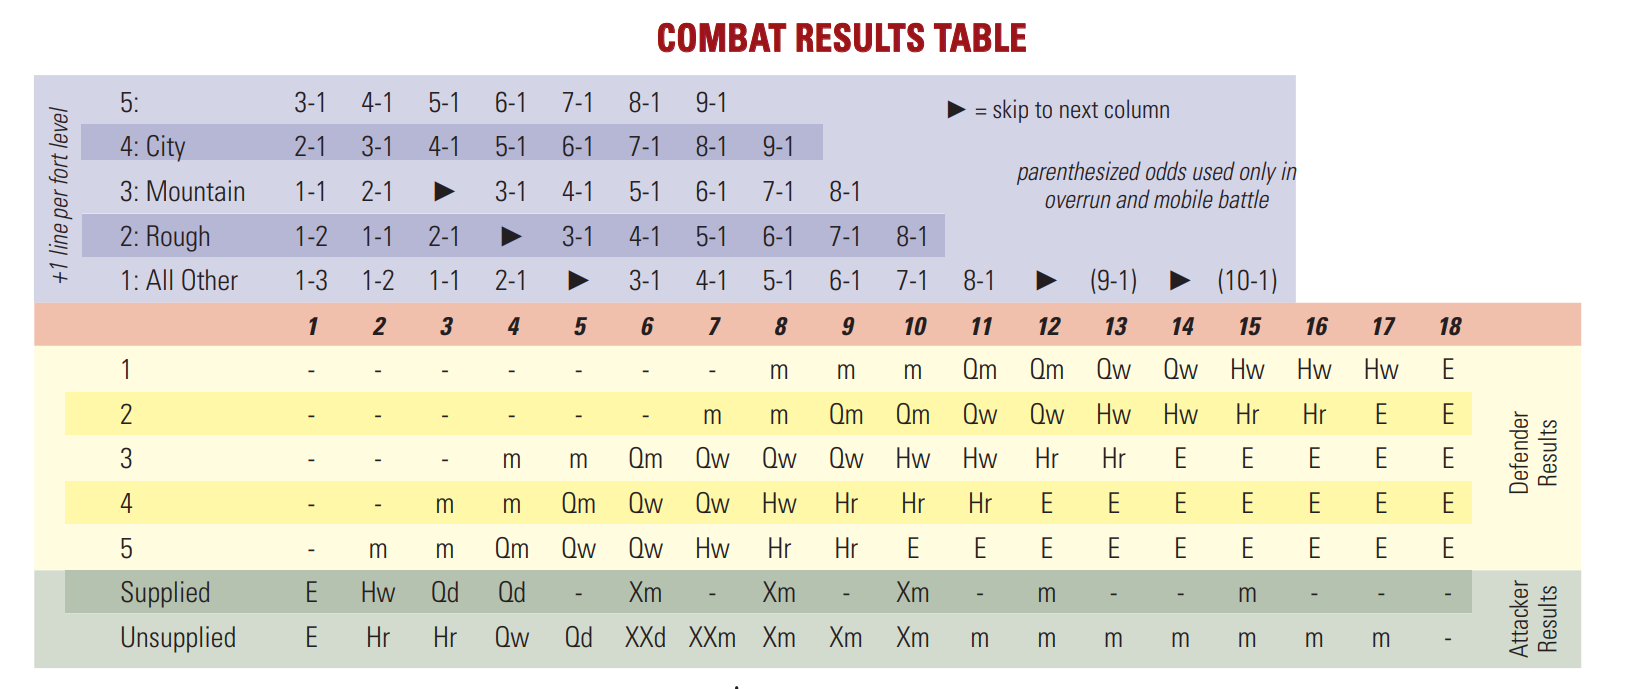
\includegraphics[scale=0.25]{data/tableau_combat.png}
\caption{Tableau du combat}
\end{figure}

Pour interpréter ce tableau il faut le diviser en trois parties distinctes. En haut la partie en bleu est la première étape.
Nous choisissons la ligne correspondant au type de terrain de l'hexagone que nous attaquons, puis on divise le nombre
d'attaquants par le nombre de défenseurs présents dans l'hexagone cible. Avec ce ratio, nous choisissons ensuite la colonne.
Ensuite nous passons a la deuxieme partie du tableau, en rouge et jaune. Avec le ratio que nous avons trouvé avant,
nous trouvons quelle colonne rouge correspond. On lance un dé (1d6) et on ajoute le résultat pour trouver la colonne finale.
Si par exemple nous étions sur la colonne 5 et le dé retourne 3, nous nous déplaçons sur la colonne 8.
Enfin pour choisir la ligne, nous prenons la valeur morale Rating de chaque défenseur, pour trouver la case correspondante.
Morale Rating est un attribut que chaque unité contient. Plus elle est petite, plus l'unité performe bien en combat.
Avec la case trouvée, on récupère deux lettres distinctes. La première représente le résultat des dégâts subits, et la deuxième le résultat du morale.
Si {\tt m} est seulement présent alors le résultat des dégâts est inexistant, et si {\tt E} alors le résultat du morale est inexistant.
Une barre signifie qu'il n'y a aucun résultat. Ces résultats sont pour les défenseurs.
Pour les attaquants, nous passons sur la dernière partie du tableau, la partie verte.
Nous gardons la même colonne qu'avant, et choisissons la ligne en dépendance de l'approvisionnement de l'attaquant.
Si il est approvisionné alors nous choisissons la ligne de haut, sinon la basse. Et recupere les resultats comme dans le cas des défenseurs.
Voici un petit tableau qui montre les résultats possibles:

\begin{figure}[H]
\centering
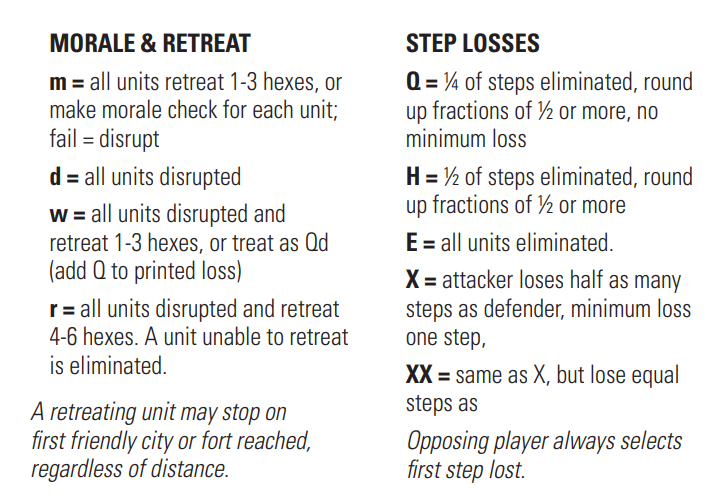
\includegraphics[scale=0.3]{data/morale_et_retraite.png}
\caption{Tableau des resultats de combat}
\end{figure}

Prenons un exemple pour mieux comprendre. Une unité A attaque une unité B. Le terrain de l'hexagone ou se trouve l'unité B est Rough, donc la ligne du tableau bleu est la deuxième.
Le ratio attaquants-défenseurs est de 1-1, car nous avons une seule unité A qui attaque une seule unité B. La colonne du tableau est alors 2.
Nous lançons un dé et le résultat est 3, donc la colonne finale est 5. Supposons que la valeur morale Rating de B est 3.
La valeur qui correspond est {\tt m}. Ceci veut dire que nous devons faire un test de morale.
Pour faire ceci nous lançons un autre dé et nous ajoutons la valeur morale Rating au résultat. Si le résultat est plus grand que 5, le test échoue.
Dans notre cas, le résultat est 4 et rien ne se passe. Passons au combattants, qui dans ce scénario
n'ont pas d'approvisionnements. La valeur de la colonne 5 pour la ligne Unsupplied est {\tt Qd}.
Donc l'unité A reçoit un quart (arrondies) de ces points de vie en dégâts et A devient {\tt disrupted}.
Supposons que A a 1 point de vie, l'arrondie de 1/4 est de 0 donc l'unité ne reçoit pas de dégât.
Avec le statut {\tt disrupted} par contre, sa valeur de morale Rating augmente de 1 et A ne pourras bouger que la moitié de son mouvement pour le reste du tour.